\documentclass[10pt]{beamer}
\usetheme[
%%% options passed to the outer theme
%    progressstyle=movCircCnt,   %either fixedCircCnt, movCircCnt, or corner
%    rotationcw,          % change the rotation direction from counter-clockwise to clockwise
%    shownavsym          % show the navigation symbols
]{AAUsimple}
  
% If you want to change the colors of the various elements in the theme, edit and uncomment the following lines
% Change the bar and sidebar colors:
%\setbeamercolor{AAUsimple}{fg=red!20,bg=red}
%\setbeamercolor{sidebar}{bg=red!20}
% Change the color of the structural elements:
%\setbeamercolor{structure}{fg=red}
% Change the frame title text color:
%\setbeamercolor{frametitle}{fg=blue}
% Change the normal text color background:
%\setbeamercolor{normal text}{fg=black,bg=gray!10}
% ... and you can of course change a lot more - see the beamer user manual.

\usepackage[utf8]{inputenc}
\usepackage[english]{babel}
\usepackage[T1]{fontenc}
% Or whatever. Note that the encoding and the font should match. If T1
% does not look nice, try deleting the line with the fontenc.
\usepackage{helvet}
\usepackage{kotex}
%\usepackage{pdftexcmds}
%\usepackage{minted}
\usepackage{pgfplots}
% colored hyperlinks
\newcommand{\chref}[2]{%
  \href{#1}{{\usebeamercolor[bg]{AAUsimple}#2}}%
}

% Added Environments

\usepackage{color}
\usepackage{fancyvrb,xcolor}% http://ctan.org/pkg/{fancyvrb,xcolor}
\DefineVerbatimEnvironment%
  {CodeVerbatim}{Verbatim}
  {formatcom=\color{red}}


\title{Welcome to Python}

\subtitle{2015 Summer Data Mining Workshop}  % could also be a conference name

%\date{\today}
\date{August 20, 2015}

\author{
  Kyunghoon Kim\\
  \href{mailto:kyunghoon@unist.ac.kr}{{\tt kyunghoon@unist.ac.kr}}
}

% - Give the names in the same order as they appear in the paper.
% - Use the \inst{?} command only if the authors have different
%   affiliation. See the beamer manual for an example

\institute[
%  {
\includegraphics[scale=0.2]{unist}}\\
  Dept.\ of Mathematical Sciences\\
  UNIST\\
  Republic of Korea
] % optional - is placed in the bottom of the sidebar on every slide
{% is placed on the bottom of the title page
  Department of Mathematical Sciences\\
  Ulsan National Institute of Science and Technology\\
  Republic of Korea
  
  %there must be an empty line above this line - otherwise some unwanted space is added between the university and the country (I do not know why;( )
}

\pgfdeclareimage[height=1.5cm]{titlepagelogo}{imgs/unist}

\titlegraphic{% is placed on the bottom of the title page
  \pgfuseimage{titlepagelogo}
%  \hspace{1cm}\pgfuseimage{titlepagelogo2}
}

\begin{document}
% the titlepage
{\aauwavesbg%
\begin{frame}[plain,noframenumbering] % the plain option removes the header from the title page
  \titlepage
\end{frame}}
%%%%%%%%%%%%%%%%

% TOC
\begin{frame}{Contents}{}
\tableofcontents
\end{frame}
%%%%%%%%%%%%%%%%

\section{Python}
\subsection{왜 프로그래밍을 배워야 하나?}
\begin{frame}{왜 프로그래밍을 배워야 하나?}{}
	\centering
	
\includegraphics[scale=0.25]{contents/program.jpg}\\
	\url{https://www.youtube.com/watch?v=nKIu9yen5nc}
\end{frame}

\subsection{왜 파이썬을 사용하나?}
\begin{frame}{왜 파이썬을 사용하나?}{}
	\centering
	\vspace{3mm}
	
\includegraphics[scale=0.51]{contents/progLanguages.jpg}\\
	\tiny{\url{http://www.collegeteacher.org/csci101/resource_programming/prog03.php}}
\end{frame}

\begin{frame}{왜 파이썬을 사용하나?}{}
	\centering
	
\includegraphics[scale=0.28]{contents/simplicity.jpg}
\end{frame}

\begin{frame}{왜 파이썬을 사용하나?}{}
	\centering
	
\includegraphics[scale=1.2]{contents/java.jpg}\\
	\tiny{\url{http://www.quora.com/Why-should-I-learn-Python-if-I-already-know-Java}}
\end{frame}

\begin{frame}{왜 파이썬을 사용하나?}{}
	\centering
	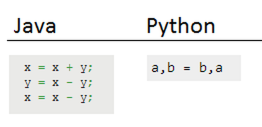
\includegraphics[scale=1]{contents/java2.png}\\
	\tiny{\url{http://www.quora.com/Why-should-I-learn-Python-if-I-already-know-Java}}
\end{frame}

\begin{frame}{왜 파이썬을 사용하나?}{}
	\centering
	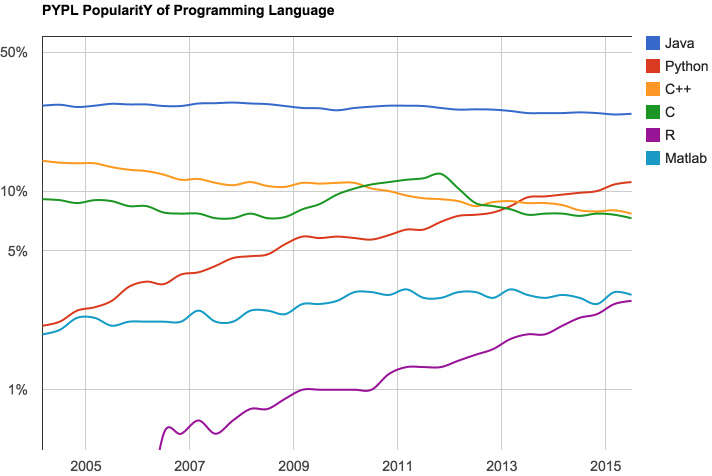
\includegraphics[scale=0.38]{contents/pypl.png}\\
	\tiny{\url{http://pypl.github.io/PYPL.html}}
\end{frame}

\begin{frame}{왜 파이썬을 사용하나?}{}
	Python is a programming language that lets you work quickly and integrate systems more effectively.
	{\centerline{
		
\includegraphics[scale=0.5]{contents/python.png}
	}}
	\\
	\url{https://www.python.org/}
\end{frame}

\subsection{어떻게 파이썬을 배우나?}
\begin{frame}{어떻게 파이썬을 배우나?}{}
	\begin{itemize}
		\item English : \url{http://code.tutsplus.com/articles/the-best-way-to-learn-python--net-26288}
		\item Korean : \url{https://nolboo.github.io/blog/2014/08/10/the-best-way-to-learn-python/}
	\end{itemize}
\end{frame}

\begin{frame}{어떻게 파이썬을 배우나?}{}
\begin{block}{Web Tutorial(links)}
	\begin{itemize}
		\item \href{https://www.codecademy.com/en/tracks/python-ko}{Codecademy python-ko}
		\item \href{http://www.pythontutor.com/visualize.html}{Python Visualization}
		\item \href{https://wakari.io/nb/url///wakari.io/static/notebooks/Lecture_1_Introduction_to_Python_Programming.ipynb}{ipython Tutorial}
		\item \href{https://www.codementor.io/learn-python-online}{Learn Python Online}
	\end{itemize}
\end{block}
\end{frame}

\begin{frame}{어떻게 파이썬을 배우나?}{}
\begin{block}{Slide(links)}
	\begin{itemize}
		\item \href{http://www.slideshare.net/MattHarrison4/learn-90?qid=14fa96b9-9b49-483d-988d-a9016e4b1f07&v=qf1&b=&from_search=1}{Learn 90\% of Python in 90 Minutes}
		\item \href{http://www.slideshare.net/blissray/w-37771905?related=1}{산업공학과를 위한 프로그래밍 입문}
	\end{itemize}
\end{block}
\end{frame}

\begin{frame}{어떻게 파이썬을 배우나?}{}
\begin{block}{Online Book(links)}
	\begin{itemize}
		\item \href{https://wikidocs.net/book/1}{점프 투 파이썬}
		\item \href{http://coreapython.hosting.paran.com/dive/chap00.html}{Dive into Python(번역본)}
		\item \href{http://coreapython.hosting.paran.com/thinkCSpy(2nd)/index.htm}{컴퓨터 과학자 같이 생각하는 법(파이썬 버전)}
		\item \href{http://interactivepython.org/runestone/static/pythonds/index.html}{Problem Solving with Algorithms and Data Structures}
		\item \href{http://coreapython.hosting.paran.com/pygnudoc.html}{파이썬 문서고}
	\end{itemize}
\end{block}
\end{frame}

\begin{frame}{어떻게 파이썬을 배우나?}{}
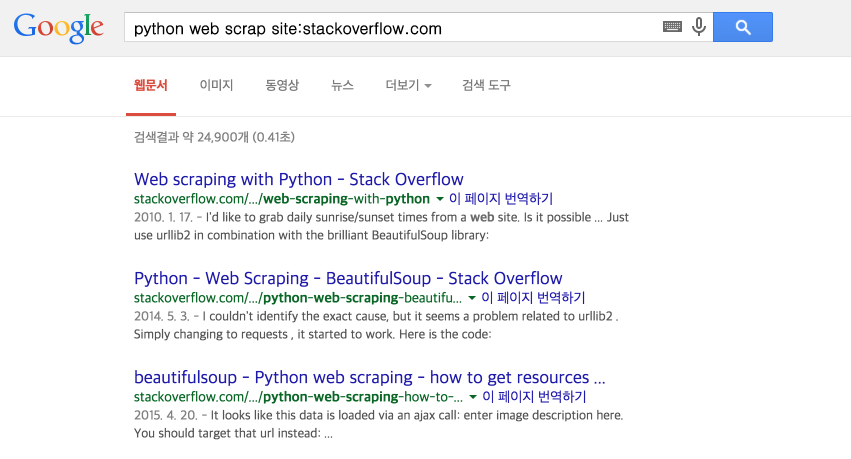
\includegraphics[scale=0.4]{contents/google.jpg}
\end{frame}

\subsection{파이썬2냐 파이썬3냐}
\begin{frame}{파이썬2냐 파이썬3냐}{}
\centering
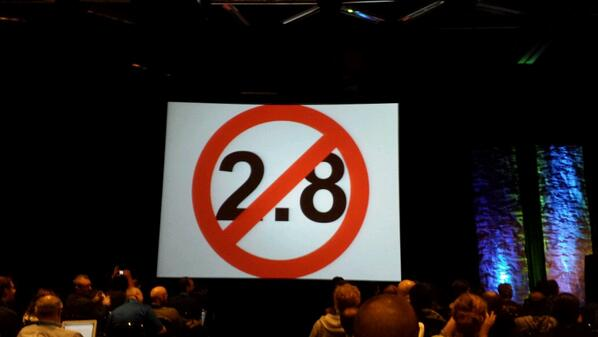
\includegraphics[scale=0.5]{contents/python28.jpg}\\
\tiny{\url{http://b.ssut.me/64}}
\end{frame}

\begin{frame}{파이썬2냐 파이썬3냐}{}
\centering
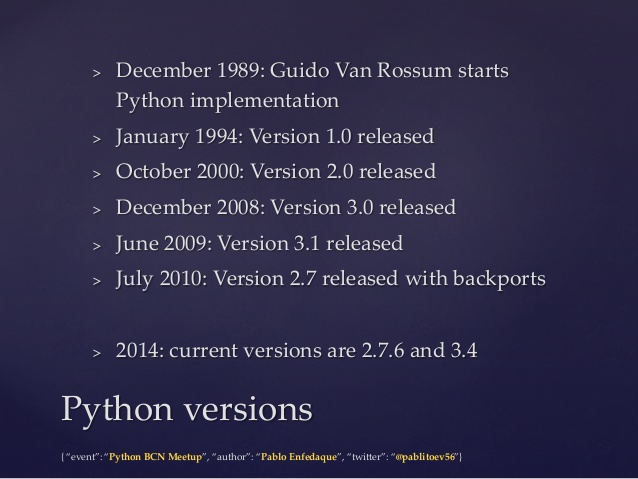
\includegraphics[scale=0.4]{contents/python23.jpg}\\
\tiny{\url{http://www.slideshare.net/pablito56/python-2-vs-python-3}}
\end{frame}

%%%%%%%%%%%%%%%%

\section{파이썬 배우기}
\subsection{파이썬 코드와 실행}
\begin{frame}[fragile]
\frametitle{파이썬 코드와 실행}
hello.py
\begin{Verbatim}[numbers=left]
print("hello world")
\end{Verbatim}
\vspace{10mm}
Command prompt
\begin{Verbatim}[numbers=left]
$ python hello.py
\end{Verbatim}

\end{frame}
%$

\subsection{객체 Object}
\begin{frame}{객체 Object}
\Large{Everything in Python is an \textbf{object}}
	\begin{itemize}
		\item identity(id)
		\item value
		\begin{itemize}
			\item mutable
			\begin{itemize}
				\item list
				\item dictionary
			\end{itemize}
			\item immutable
			\begin{itemize}
				\item string
				\item integer
				\item tuple
			\end{itemize}
		\end{itemize}
	\end{itemize}
\end{frame}

\subsection{help(), dir()}
\begin{frame}[fragile]
\frametitle{help(), dir()}
정의된 객체에 관한 문서를 얻을 때 사용하는 명령어.\\
\begin{block}{1. help()}
	객체에 대해 뭔가 알고 싶다
\end{block}
\begin{Verbatim}[numbers=left,commandchars=\\\{\}]
>>> help(dir)
Help on built-in function dir in module __builtin__:

dir(...)
    dir([object]) -> list of strings
\end{Verbatim}
\begin{block}{2. dir()}
	객체의 속성에 관한 목록을 얻고 싶다
\end{block}
\begin{Verbatim}[numbers=left,commandchars=\\\{\}]
>>> dir(help)
[`__call__', `__class__', `__delattr__', `__dict__', ...]
\end{Verbatim}
\end{frame}

\subsection{변수의 자료형}
\begin{frame}[fragile]
\frametitle{변수의 자료형}
변수는 자료형이 없어서 선언할 필요가 없다.
\begin{Verbatim}[numbers=left,commandchars=\\\{\}]
>>> a = 3 # integer
>>> b = 3.14 # float
>>> c = "string" # string
>>> d = `string'
>>> e = "3"
\end{Verbatim}
\vspace{5mm}
\begin{Verbatim}[numbers=left,commandchars=\\\{\}]
>>> type(a)
int
>>> type(b)
float
>>> type(c)
str
\end{Verbatim}
\end{frame}

\begin{frame}[fragile]
\frametitle{정수의 자료형}
고정 소수점 Fixed point 방식\\
\vspace{10mm}
\textbf{int} : 마이크로프로세서의 기본 비트의 길이
\begin{Verbatim}[numbers=left,commandchars=\\\{\}]
>>> import sys
>>> print(sys.maxint)
9223372036854775807
\end{Verbatim}
\vspace{10mm}
\textbf{long} : 정수의 범위를 넘어서는 큰 숫자(only python2)
\begin{Verbatim}[numbers=left,commandchars=\\\{\}]
>>> print(sys.maxint+1)
9223372036854775808L
\end{Verbatim}
\end{frame}

\begin{frame}[fragile]
\frametitle{실수의 자료형}
부동 소수점 Floating point 방식\\
\small{: 소수점의 위치를 고정하지 않고 그 위치를 나타내는 수(exponent)를 따로 적음}\\
\begin{equation*}
[mantissa]*[base]^{[exponent]}
\end{equation*}
\vspace{10mm}
정밀도 precision 문제 발생
\begin{Verbatim}[numbers=left,commandchars=\\\{\}]
>>> (1234.567+0.001)+0.0004
1234.5683999999999
\end{Verbatim}
\vspace{5mm}
\begin{Verbatim}[numbers=left,commandchars=\\\{\}]
>>> 1234.567+(0.001+0.0004)
1234.5684
\end{Verbatim}
\end{frame}

\begin{frame}[fragile]
\frametitle{정밀도 설정}
decimal 객체를 생성하여 10진수를 정확하게 나타낼 수 있음.\\
\vspace{2mm}
\begin{Verbatim}[numbers=left,commandchars=\\\{\}]
>>> from decimal import Decimal, getcontext # Module import
>>> getcontext().prec = 12 # precision
>>> Decimal(1234.567)+Decimal(0.001)+Decimal(0.0004)
Decimal(`1234.56840000')
>>> getcontext().prec = 24
>>> (Decimal(1234.567)+Decimal(0.001))+Decimal(0.0004)
Decimal(`1234.56840000000000727600')
>>> Decimal(1234.567)+(Decimal(0.001)+Decimal(0.0004))
Decimal(`1234.56840000000000727600')
>>> Decimal(10)**600
Decimal('1.00000000000000000000000E+600')
\end{Verbatim}
\vspace{2mm}
하지만.. 긴 시간의 연산에서는 느리다.
\end{frame}

\begin{frame}[fragile]
\frametitle{정수의 나눗셈}
\begin{Verbatim}[numbers=left,commandchars=\\\{\}]
>>> 3/4
0
>>> 3/4.
0.75
\end{Verbatim}
\vspace{2mm}
Python3에서는 문제가 없다.
\end{frame}

\begin{frame}[fragile]
\frametitle{복소수}
실수, 허수 부분은 64비트 부동 소수점 숫자로 저장됨.
\begin{Verbatim}[numbers=left,commandchars=\\\{\}]
>>> a = 1-2j
>>> a.real
1.0
>>> a.imag
-2.0
>>> abs(a)
2.23606797749979
>>> a
(1-2j)
\end{Verbatim}
\end{frame}

\begin{frame}[fragile]
\frametitle{문자열}
\begin{Verbatim}[numbers=left,commandchars=\\\{\}]
>>> a = `apple'
>>> b = "apple"
>>> c = """apple"""
>>> print a, b, c
apple apple apple
\end{Verbatim}
\vspace{2mm}
String Escaping
\begin{Verbatim}[numbers=left]
>>> print "I'm happy"
I'm happy
>>> print `I\'m happy'
I'm happy
>>> print """\"I'm happy\""""
"I'm happy"
\end{Verbatim}
\end{frame}

\begin{frame}[fragile]
\frametitle{문자열 포맷}
\begin{Verbatim}[numbers=left,commandchars=\\\{\}]
>>> a = "apple"
>>> b = "banana"
>>> "%s and %s" % (a, b)
`apple and banana'
>>> "{0} and {1}".format(a, b)
`apple and banana'
>>> print a, "and", b
apple and banana
\end{Verbatim}
\end{frame}

\begin{frame}[fragile]
\frametitle{문자열 방법}
Dunder(Double under) Methods and String Methods
\begin{Verbatim}[numbers=left,commandchars=\\\{\}]
>>> dir("apple")
['__add__', '__class__', '__contains__', '__delattr__',
'__doc__', '__eq__', '__format__', '__ge__', '__getattribute__',
...
'capitalize', 'center', 'count', 'decode', 'encode',
'endswith', 'expandtabs', 'find', 'format', 'index',
'isalnum', 'isalpha', 'isdigit', 'islower', 'isspace',
'istitle', 'isupper', 'join', 'ljust', 'lower', 'lstrip',
'partition', 'replace', 'rfind', 'rindex', 'rjust',
'rpartition', 'rsplit', 'rstrip', 'split', 'splitlines',
'startswith', 'strip', 'swapcase', 'title', 'translate',
'upper', 'zfill']
\end{Verbatim}
\end{frame}

\subsection{주석 comment}
\begin{frame}[fragile]
\frametitle{주석 comment}
\begin{Verbatim}[numbers=left,commandchars=\\\{\}]
# 한 줄 주석

"""
여러 줄 주석
"""
\end{Verbatim}
\end{frame}

\begin{frame}{그 외 자료형들}
\begin{itemize}
\item None
\item Booleans
\item Sequences
	\begin{itemize}
		\item list
		\item tuple
		\item set
	\end{itemize}
\item Dictionary
\end{itemize}
\end{frame}

\subsection{리스트 list}
\begin{frame}[fragile]
\frametitle{리스트 list}
\begin{Verbatim}[numbers=left,commandchars=\\\{\}]
>>> a = ['apple', 'banana', 'kiwi']
>>> a[0]
'apple'
>>> a[2]
'kiwi'
>>> a[-1] # a[len(a)-1]
'kiwi'
>>> len(a)
3
\end{Verbatim}
\end{frame}

\begin{frame}[fragile]
\frametitle{리스트 list}
\begin{Verbatim}[numbers=left,commandchars=\\\{\}]
>>> dir([])
[..., 'append', 'count', 'extend', 'index',
'insert', 'pop', 'remove', 'reverse', 'sort']

>>> a.append('melon')
>>> a
['apple', 'banana', 'kiwi', 'melon']
>>> a.index('kiwi')
2
>>> a.remove('banana')
>>> a
['apple', 'kiwi', 'melon']
>>> a.pop(2)
'melon'
>>> a
['apple', 'kiwi']
\end{Verbatim}
\end{frame}

\begin{frame}[fragile]
\frametitle{리스트 list}
\begin{Verbatim}[numbers=left,commandchars=\\\{\}]
>>> range(10) # half-open interval
[0, 1, 2, 3, 4, 5, 6, 7, 8, 9]
>>> range(3, 10) # length = end - start
[3, 4, 5, 6, 7, 8, 9]
>>> range(1, 10, 2)
[1, 3, 5, 7, 9]
>>> a = range(10)
>>> a
[0, 1, 2, 3, 4, 5, 6, 7, 8, 9]
>>> a[3:5]
[3, 4]
>>> a[::-1]
[9, 8, 7, 6, 5, 4, 3, 2, 1, 0]
\end{Verbatim}
\end{frame}

\subsection{사전 dictionary}
\begin{frame}[fragile]
\frametitle{사전 dictionary}
Hashmap, Associative array
\begin{Verbatim}[numbers=left]
>>> a = {} # a = dict()
>>> a['apple'] = 500
>>> a['banana'] = 200
>>> a
{'apple': 500, 'banana': 200}
\end{Verbatim}
\vspace{2mm}
\begin{Verbatim}[numbers=left]
>>> dir({})
[...,'clear', 'copy', 'fromkeys', 'get', 'has_key', 'items',
'iteritems', 'iterkeys', 'itervalues', 'keys', 'pop',
'popitem', 'setdefault', 'update', 'values', 'viewitems',
'viewkeys', 'viewvalues']
\end{Verbatim}
\end{frame}

\begin{frame}[fragile]
\frametitle{사전 dictionary}
\begin{Verbatim}[numbers=left]
>>> apple = dict()
>>> apple = {"price": 500, "type": ["fruit", "red"],
    "property": {"a": 1}}
>>> apple['price']
500
>>> apple['type']
['fruit', 'red']
>>> apple['type'][0]
'fruit'
>>> apple['property']
{'a': 1}
>>> apple['property']['a']
1
>>> apple.get("price", None)
500
>>> apple.get("where", None)
>>>
\end{Verbatim}
\end{frame}

\begin{frame}[fragile]
\frametitle{그 외 유용한 자료형들}
\begin{Verbatim}[numbers=left]
>>> values = [1,1,1,2,3,3,4,5,6,7,7]
>>> set(values) # 집합 set
set([1, 2, 3, 4, 5, 6, 7])
>>> list(set(values))
[1, 2, 3, 4, 5, 6, 7]
\end{Verbatim}
\vspace{2mm}
\begin{Verbatim}[numbers=left]
>>> a = (11, 23, "Monday") # 튜플 tuple
>>> (mon, day, text) = a
>>> print mon, day, text
11 23 Monday
\end{Verbatim}
\end{frame}

\section{함수 Function}
\begin{frame}[fragile]
\frametitle{함수 Function}
\begin{equation*}
f(x) = 4x*(1-x)
\end{equation*}
\begin{Verbatim}[numbers=left,commandchars=\\\{\}]
>>> def f(x):
        return 4*x*(1-x)
>>> f(0.2)
0.6400000000000001
\end{Verbatim}
\end{frame}

\begin{frame}[fragile]
\frametitle{함수 Function}
\begin{Verbatim}[numbers=left,commandchars=\\\{\}]
>>> from decimal import Decimal, getcontext
>>> getcontext().prec = 24
>>> def f(a, x):
        """ Logistic Function """
        x = Decimal(x)
        return a*x*(1-x)
>>> f(4, 0.2)
Decimal('0.640000000000000026645353')

>>> help(f)
Help on function f in module __main__:

f(a, x)
    Logistic Function
\end{Verbatim}
\end{frame}

\section{반복문 Loop statement}
\begin{frame}[fragile]
\frametitle{반복문 Loop}
\begin{Verbatim}[numbers=left]
>>> for i in ['apple', 'banana', 'kiwi']:
...     print i
...
apple
banana
kiwi

>>> for i in range(0, 10, 2):
...     print i
...
0
2
4
6
8
\end{Verbatim}
\end{frame}

\begin{frame}[fragile]
\frametitle{반복문 Loop}
\begin{Verbatim}[numbers=left]
>>> x = 0.1
>>> for i in range(10):
        print x
        x = f(4, x) # logistic function
    print x
0.1
0.360000000000000017763568
0.921600000000000019895195
0.289013759999999932897486
0.821939226122649486738340
0.585420538734198249301121
0.970813326249437346212131
0.113339247303763482961149
0.401973849297519300076195
0.961563495113818170323396
0.147836559913265400036406
\end{Verbatim}
\end{frame}

\section{조건문 Conditional statement}
\begin{frame}[fragile]
\frametitle{조건문 Conditional statement}
\begin{Verbatim}[numbers=left]
>>> x = 0.1
>>> for i in range(100):
        print x
        x = f(2, x)
    print x
0.1
0.180000000000000008881784
0.295200000000000011368684
0.416113920000000009313226
0.485926251164467203125000
0.499603859187428678487954
0.499999686144913230666241
0.499999999999802989969018
0.500000000000000000000000
0.500000000000000000000000
0.500000000000000000000000
0.500000000000000000000000
\end{Verbatim}
\end{frame}

\begin{frame}[fragile]
\frametitle{조건문 Conditional statement}
\begin{Verbatim}[numbers=left]
>>> x = Decimal(0.1)
>>> for i in range(100):
        print x
        new_x = f(2, x)
        if new_x - x < 0.0000001:
            print "Converged"
            break
        else:
            x = new_x
    print x
0.1000000000000000055511151231257827021181583404541015625
0.180000000000000008881784
0.295200000000000011368684
0.416113920000000009313226
0.485926251164467203125000
0.499603859187428678487954
0.499999686144913230666241
0.499999999999802989969018 Converged
\end{Verbatim}
\end{frame}

\begin{frame}[fragile]
\frametitle{조건문 Conditional statement}
\begin{Verbatim}[numbers=left]
>>> A = 85
>>> if A>90:
...     print "A"
... elif A>80:
...     print "B"
... elif A>70:
...     print "C"
... else:
...     print "D"
...
B
\end{Verbatim}
\end{frame}

\begin{frame}[fragile]
\frametitle{반복문과 조건문 예}
\begin{Verbatim}[numbers=left]
>>> animals = ['cat', 'dog', 'cock', 'rabbit']
>>> for index, value in enumerate(animals):
...     print index, value
...
0 cat
1 dog
2 cock
3 rabbit

>>> for index, value in enumerate(animals):
...     if value[0] == 'c':
...         print index, value
...
0 cat
2 cock
\end{Verbatim}
\end{frame}

\section{클래스 Class}
\begin{frame}[fragile]
\frametitle{클래스 Class}
\begin{itemize}
	\item object
	\item constructor(dunder init)
	\item All method take \textbf{self} as first parameter.
\end{itemize}
\vspace{2mm}
\begin{Verbatim}[numbers=left,commandchars=\\\{\}]
>>> class Animal(object):
...     def __init__(self, name):
...         self.name = name
...     def talk(self):
...         print "Hello"
...
>>> animal = Animal('thing')
>>> animal.talk()
Hello
\end{Verbatim}
\end{frame}

\begin{frame}[fragile]
\frametitle{서브클래스 Subclass}
\begin{Verbatim}[numbers=left,commandchars=\\\{\}]
>>> class Cat(Animal):
...     def talk(self):
...         print "%s is cat name." % (self.name)
...
>>> cat = Cat("Persia")
>>> cat.talk()
Persia is cat name.
\end{Verbatim}
\end{frame}

%\begin{frame}[fragile]
%\frametitle{}
%\begin{Verbatim}[numbers=left,commandchars=\\\{\}]
%\end{Verbatim}
%\end{frame}
%
%\begin{frame}[fragile]
%\frametitle{}
%
%\end{frame}
%
%\begin{frame}[fragile]
%\frametitle{}
%
%\end{frame}


%%%%%%%%%%%%%%%%

{\aauwavesbg
\begin{frame}[plain,noframenumbering]
  \finalpage{
  \Large{Thank you for attention!}
  \\
  \vspace{2mm}
  \small{In case you have any comments, suggestions or have found a bug, please do not hesitate to contact me.}
  \begin{center}
    \insertauthor\\
    Graduate Student in\\
    Computational Mathematical Sciences Laboratory
    \url{http://amath.unist.ac.kr}
  \end{center}}
\end{frame}}
%%%%%%%%%%%%%%%%

\end{document}
